\documentclass{article}

%%% Fill details here (in the second brackets)
\newcommand{\name}{Weijie Gan}     % Your name (First Last)
\newcommand{\wustlkey}{gan.weijie}          % Your WUSTL Key
%%%



%%%%%%%%%%%%%%%%%%%%%% Formatting Stuff %%%%%%%%%%%%%%%%%%%%%%%%%%%
\usepackage{times}
\usepackage[T1]{fontenc}

\setlength{\parskip}{1em}\setlength{\parindent}{0pt}
\linespread{1.25}
\usepackage[margin=0.7in,top=1in]{geometry}\usepackage{fancyhdr}
\pagestyle{fancy}\lhead{\bf \name}\rhead{\bf \wustlkey}\cfoot{\thepage}
\newcommand{\info}{\clearpage \subsection*{Information}}
\newcommand{\solution}[1]{\clearpage \subsection*{Solution #1}}
\newcommand{\spart}[1]{\paragraph{(#1)}}
%%%%%%%%%%%%%%%%%%%%%%%%%%%%%%%%%%%%%%%%%%%%%%%%%%%%%%%%%%%%%%%%%%%


%%% Add any more packages if you want to
\usepackage{amsmath,graphicx}


\begin{document}
%%%%% Main Body goes here

% Begin solution to every problem like this.
\solution{1} 

\spart{a} The vertically flipped image is shown in Figure \ref{fig:vert}.

\begin{figure*}[!h]
  \centering
  
\includegraphics[height=5em]{./code/outputs/flipy.jpg}
  \caption{Vertically flipped image for problem 1.}
  \label{fig:vert}
\end{figure*}

\spart{b} The horizontally flipped image is shown in Figure \ref{fig:horiz}.

\begin{figure*}[!h]
  \centering
  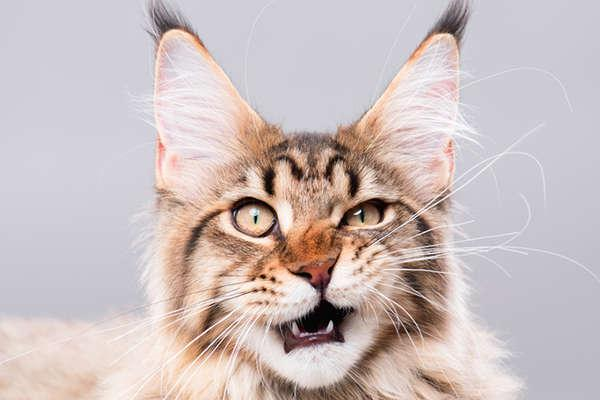
\includegraphics[height=5em]{./code/outputs/flipx.jpg}
  \caption{Horizontally flipped image for problem 1.}
  \label{fig:horiz}
\end{figure*}

%%%%%%%%%% Important, you must edit and complete the informational
%%%%%%%%%% section below. If you discussed the problem set with no
%%%%%%%%%% one, edit it to say no discussions or external resources.
\info

This problem set took approximately 0.1 hours of effort.

% I discussed this problem set with:
% \begin{itemize}
% \item A
% \item B
% \item C
% \end{itemize}

% Note that you might have to escape some special symbols in URLS like \_
% I also got hints from the following sources:
% \begin{itemize}
% \item Wikipedia article on matrix calculus at https://en.wikipedia.org/wiki/Matrix\_calculus
% \item Read numpy tutorial from https://docs.scipy.org/doc/numpy-1.13.0/user/basics.broadcasting.html
% \end{itemize}

\end{document}
